\documentclass[11pt,a4paper]{article}
%\documentclass[11pt,a4paper]{scrartcl}
%\documentclass[11pt,a4paper,oneside]{book}
\usepackage[british,UKenglish,USenglish,english,american]{babel}
%\usepackage[a4paper, total={16cm, 23cm}]{geometry}
\usepackage[tmargin = 1.25in,bmargin = 1.25in,lmargin = 1in,rmargin = 
1in]{geometry}
\usepackage{tikz}
\usepackage{graphicx}
\usepackage{pgfplots}
\pgfplotsset{width=12cm,compat=1.9}
\usepackage{setspace}
\usepackage{chemmacros}
\usepackage{chemfig}
%\usepackage{ghsystem}
%\usechemmodule{redox}
%\usepackage{chemnum}
%\usepackage{bohr}
%\usepackage{elements}
%\usepackage{endiagram}
%\usepackage{modiagram}
%\usepackage{chemgreek}
%\usepackage{mhchem}
\usepackage{esint}
\usepackage{tabularray}

\usepackage{makeidx}
\usepackage{epstopdf}

\usepackage{amssymb}
\usepackage{mathrsfs}
%\usepackage{minted}
\usepackage{bm}
\usepackage{amsmath}
\usepackage{enumitem}
\usepackage[english]{varioref}
\usepackage[english]{babel}
\usepackage{lipsum}
\usepackage{fancyhdr}
\pagestyle{fancy} 
\usepackage{float}
\usepackage{empheq}
\usepackage[framemethod=tikz]{mdframed}
\usepackage{epstopdf}
\numberwithin{equation}{section}
\usepackage{eso-pic}
\usepackage{calc}
\usepackage{nccmath}
\usepackage{caption}
\usepackage{subcaption}
\usepackage{gensymb}
\usepackage{amsfonts,amsthm,epsfig,epstopdf,titling,url,array}
\usepackage{siunitx}
\sisetup{input-digits = 0123456789\pi}
\usepackage[symbol]{footmisc}
\usepackage{xcolor}
\usepackage{multicol}
\usepackage{boondox-cal}
\DeclareSIUnit\atm{atm}
\setcounter{secnumdepth}{3}
\setcounter{tocdepth}{3}
\usepackage{booktabs}
\usepackage{blindtext}
\usepackage{changepage}

% \usepackage{draftwatermark}
% \SetWatermarkText{DRAFT}
% \SetWatermarkScale{5}

\DeclareSIUnit\atm{atm}

\fancypagestyle{firstpage}{
	\rhead{
%		\begin{picture}(0,0) \put(-30,0){
\includegraphics[width=1cm]{figures/MCI_4C_bw.eps}} \end{picture}
	}
}
\fancyhead[L]{\slshape\nouppercase{\leftmark}}
\chead{}
\rhead{
%	\begin{picture}(0,0) \put(-30,0){
\includegraphics[width=1cm]{figures/MCI_4C_bw.eps}} \end{picture}
}
\lfoot{\textit{}}
\cfoot{-\ \thepage\ -}
\rfoot{\textit{}}
\renewcommand{\headrulewidth}{0.4pt}
\renewcommand{\footrulewidth}{0.4pt}
\newcommand{\abs}[1]{\left|#1\right|}
\definecolor{mycolor1}{rgb}{0.95, 0.95, 0.95}
\definecolor{mycolor2}{rgb}{0.95, 0.95, 0.95}
\definecolor{tableShade}{gray}{0.9}
\newcommand{\sign}{\text{sign}}
\newcommand{\centered}[1]{\begin{tabular}{@{}l@{}} #1 \end{tabular}}
\theoremstyle{it}
\newtheorem{defn}{Definition}[section]
\newtheorem{thm}{Theorem}[section]
\theoremstyle{definition}
\newtheorem{example}{Example}[section]

\newenvironment{myitemize_1}
{ \begin{itemize}[topsep=0pt]
		\setlength{\topsep}{2pt}		
		\setlength{\itemsep}{2pt}
		\setlength{\parskip}{2pt}
		\setlength{\parsep}{2pt}     }
	{ \end{itemize}                  }


\newmdenv[innerlinewidth=0.5pt, roundcorner=4pt,backgroundcolor=mycolor2, linecolor=mycolor1,innerleftmargin=6pt,
innerrightmargin=6pt,innertopmargin=6pt,innerbottommargin=6pt]{mybox}

\title{\textbf{ 
		\begin{LARGE}
			Permanent Magnet Synchronous Machine
		\end{LARGE} \\[24pt]
		\begin{Large}
			Model and Control Strategies  
	\end{Large}}
}
\author{\textbf{Davide Bagnara}}

\begin{document}
	\begin{onehalfspace}
	\thispagestyle{firstpage}
	\begin{mybox}
		\maketitle
		\vspace{125mm}
	\end{mybox}
	\newpage
	\tableofcontents
	\listoffigures	
	\listoftables
	\newpage
	
	{In this document, the permanent magnet synchronous machine (pmsm) and its generic vector control are shown. The pmsm, implemented into the \textit{Simscape} model, has been presented in machine variables (uvw). The following document will cover either representations $\alpha\beta$ (stationary) and dq (rotating) which are extensively used as model base for control and state observers design. Additional topics like MTPA (max torque per ampere), FW (field weakening) and per unit normalization will be taken into account. 
		
	\noindent The following arguments will be presented:
	\begin{itemize}
		\item[$-$] \textbf{PMSM model derivation for different reference frames and machine variables representation.}
		\item[$-$] \textbf{Basic vector control description.}
		\begin{itemize}
			\item[$-$] Normalization of the motor quantities.
			\item[$-$] Speed control.
			\item[$-$] Torque (vector current) control.
			\item[$-$] Max torque per ampere.
			\item[$-$] Field weakening.
		\end{itemize}
		\item[$-$] \textbf{Parameters identification from common data-sheet.}
		\item[$-$] \textbf{Parameters setting.}
		\item[$-$] \textbf{Model output variables.}
\end{itemize}}


\section{PMSM machine based model derivation}
In this section the PMSM model in machine coordinates is derived. The developed model is used as physical model in the \textit{Simscape} environment.

We can summarize the PMSM as a rotating permanent magnet coupled to three $120\degree$ shifted coils. During the rotation the time derivative of the magnetic flux linkages to the coils induces an electromagnetic force (emf) into the coils as $$e(t) = -\frac{d\psi^r(t)}{dt}$$.
hence we can write the following generalized voltage Kirchhoff's law equations
\begin{equation}\label{threephase_eq1}
	\left\lbrace \begin{aligned}
		& \vec{u}_{uvw}-\mathbf{R}\vec{i}_{uvw}-\frac{d\vec{\psi}^s_{uvw}}{dt} = 0 \\[6pt]
		& J\dot{\omega}_m = \tau_m-\tau_l \\[6pt]
		& \dot{\theta} = \omega = p\omega_m
	\end{aligned} \right. 
\end{equation}
where $\vec{u}_{uvw}=\begin{bmatrix} u_u(t) &  u_v(t) & u_w(t) \end{bmatrix}^T$, $\vec{i}_{uvw}=\begin{bmatrix} i_u(t) &  i_v(t) & i_w(t) \end{bmatrix}^T$ are the three phase voltage and current vector. The magnetic flux $\vec{\psi}^s_{uvw}=\begin{bmatrix} \psi_u^s(t) &  \psi_v^s(t) & \psi_w^s(t) \end{bmatrix}^T$ represents the stator magnetic flux linkages and $p$ is the number of pole-pairs.

Recall that 
\begin{equation*}
	\vec{u}_{uvw}^s-\mathbf{R}\vec{i}_{uvw}^s-\frac{d\vec{\psi}^s_{uvw}}{dt} = 0 \leftrightarrow
	\vec{u}_{uvw}-\mathbf{R}\vec{i}_{uvw}-\frac{d\vec{\psi}^s_{uvw}}{dt} = 0
\end{equation*}
The flux linkages may be written as

\begin{equation}\label{threephase_eq2}
	\begin{aligned}
		\vec{\psi}^s_{uvw} = \mathbf{L}_s\vec{i}_{uvw}+\vec{\psi}^{\,r}_{uvw}
	\end{aligned}
\end{equation}
where $\vec{\psi}^{\,r}_{uvw}$ are the rotor flux linked to the stator generated by the rotor permanent magnets and where
\begin{equation}\label{Leq}
	\mathbf{L}_s = 
	\begin{bmatrix} 
		L_{\mu}+L_a-L_b\cos2\theta & -\frac{1}{2}L_a-L_b\cos2(\theta-\frac{\pi}{3}) & -\frac{1}{2}L_a-L_b\cos2(\theta+\frac{\pi}{3}) \\[6pt]
		-\frac{1}{2}L_a-L_b\cos2(\theta-\frac{\pi}{3}) & L_{\mu}+L_a-L_b\cos2(\theta-\frac{2\pi}{3}) & -\frac{1}{2}L_a-L_b\cos2(\theta+\pi) \\[6pt]
		-\frac{1}{2}L_a-L_b\cos2(\theta+\frac{\pi}{3}) & -\frac{1}{2}L_a-L_b\cos2(\theta+\pi) & L_{\mu}+L_a-L_b\cos2(\theta+\frac{2\pi}{3})
	\end{bmatrix}
\end{equation}
is the stator inductance matrix. $L_b$ is the anisotropic inductance term which is characteristic of internal permanent magnet machines. 
\begin{figure}[H]
	\centering
	\includegraphics[width = 0.5\textwidth, width = 240pt, keepaspectratio]{figures/pmsm/electrical_three_phases.eps}
	\captionsetup{width=0.5\textwidth, font=small} 
	\caption	{Stationary and rotating reference frame}
	\label{electrical_three_phase}
\end{figure}
In case of isotropic machine construction this term is null and the matrix of Eq.~\eqref{Leq} becomes
\begin{equation}
	\mathbf{L}_s = 
	\begin{bmatrix} 
		L_{\mu}+L_a & -\frac{1}{2}L_a & -\frac{1}{2}L_a \\[6pt]
		-\frac{1}{2}L_a & L_{\mu}+L_a & -\frac{1}{2}L_a \\[6pt]
		-\frac{1}{2}L_a & -\frac{1}{2}L_a & L_{\mu}+L_a
	\end{bmatrix} =
	\begin{bmatrix} 
		L_s & L_m & L_m \\[6pt]
		L_m & L_s & L_m \\[6pt]
		L_m & L_m & L_s
	\end{bmatrix}
\end{equation}
Where the term $L_{\mu}$ is the leakage inductance and in general can be considered between one tenth and one twentieth of the synchronous inductance, that means $L_s \approx L_a$. $L_m$ is the mutual inductance and is defined as negative value.

\begin{equation}\label{threephase_eq3}
	\left\lbrace \begin{aligned}
		& \vec{u}_{uvw}-\mathbf{R}\vec{i}_{uvw}-\omega\frac{d\mathbf{L}_s}{d\theta}\vec{i}_{uvw}-\mathbf{L}_s\frac{d\vec{i}_{uvw}}{dt}-\frac{d\vec{\psi}^{\,r}_{uvw}}{dt} = 0 \\[6pt]
		& J\dot{\omega}_m = \tau_m-b{\omega}_m-\tau_l \\[6pt]
		& \dot{\vartheta} = \omega =p\omega_m
	\end{aligned} \right. 
\end{equation}
where
\begin{equation}\label{magnet_flux}
	\left\lbrace \begin{aligned}
		\psi_u^r(t) &= \psi^m\cos(\theta) \\[6pt]
		\psi_v^r(t) &= \psi^m\cos(\theta-\frac{2\pi}{3}) \\[6pt]
		\psi_w^r(t) &= \psi^m\cos(\theta+\frac{2\pi}{3})
	\end{aligned} \right. 
\end{equation}
where $\vec{\psi}^{\,r}_{uvw}$ is the flux linkage and where $\psi^m$ is the amplitude of the flux linkages generated by the permanent magnet. In other words, $d\vec{\psi}^{\,r}_{uvw}/dt$ would be the open-circuit voltage induced in each stator phase winding. 

The expression of the electromagnetic torque may be written in machine variables using
\begin{align}\label{electromagnetic_torque_machine_variables_1}
	\tau_m(t) = p\frac{\partial W_c}{\partial \vartheta}
\end{align}
where $p$ is the number of pole pairs and
\begin{align}\label{electromagnetic_torque_machine_variables_2}
	W_c = \frac{1}{2}\vec{i}_{uvw}^{\,T}\mathbf{L}_s\vec{i}_{uvw}+\vec{i}_{uvw}^{\,T}\vec{\psi}^{\,r}_{uvw}+W_{pm}
\end{align}
In Eq.~\ref{electromagnetic_torque_machine_variables_1}, $W_{pm}$ is the energy in the coupling field due to the presence of the permanent magnet. Substituting Eq.~\ref{electromagnetic_torque_machine_variables_2} into Eq.~\ref{electromagnetic_torque_machine_variables_1} and neglecting any change in $W_{pm}$ with rotor position, the electromagnetic torque is expressed
\begin{equation}\label{electromagnetic_torque_machine_variables_3}
	\begin{aligned}
		\tau_m(t) = -p&\Big\{\frac{L_d-L_q}{3}\Big[\Big(i_u^2-\frac{1}{2}i_v^2-\frac{1}{2}i_w^2 -i_ui_v-i_ui_w+2i_vi_w\Big)\sin2\vartheta \\[6pt]
		&+\frac{\sqrt{3}}{2}\big(i_v^2-i_w^2-2i_ui_v+2i_ui_w\big)\cos2\vartheta\Big] \\[6pt]
		&+ \psi^m\Big[\Big(i_u-\frac{1}{2}i_v-\frac{1}{2}i_w\Big)\sin\vartheta - \frac{\sqrt{3}}{2}\big(i_v-i_w\big)\cos\vartheta\Big]\Big\}
	\end{aligned}
\end{equation}
where 
\begin{align}
	L_q = \frac{3}{2}\Big(L_a+L_b\Big) \\[6pt]
	L_d = \frac{3}{2}\Big(L_a-L_b\Big)
\end{align}

\section{PMSM control based model derivation}
\subsection{PMSM model respect to a stationary reference frame}
The system which we are considering is a 3-wire circuit that means we can apply the Kirchhoff condition $x_a+x_b+x_c=0$ that means we have three (not independent) vectors which lay in a plane (2-dimensions), hence the whole three phase system can be represented by the use of only one independent vector and can be represented by two coordinates $(\alpha,\beta)$.
\begin{figure}[H]
	\centering
	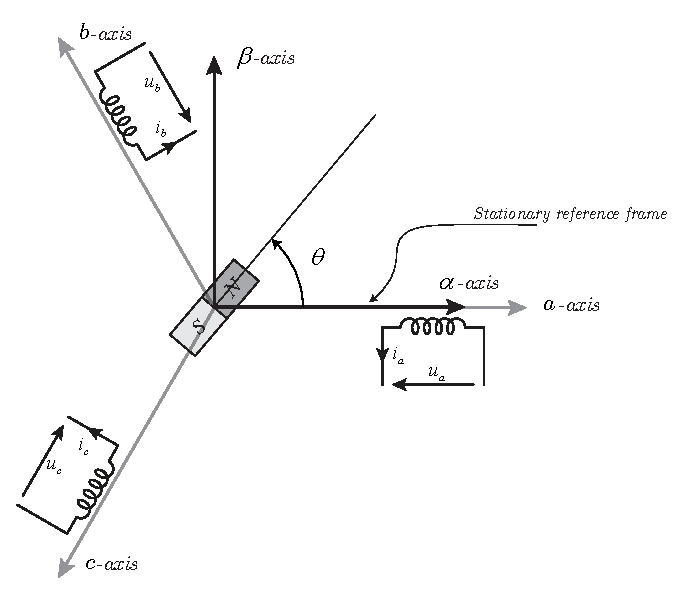
\includegraphics[width = 260pt, keepaspectratio]{figures/pmsm/reference_frames_ab.eps}
	\captionsetup{width=0.5\textwidth, font=small} 
	\caption	{Stationary $\alpha\beta$ reference frame}
	\label{figure:reference_frames}
\end{figure}
Applying the coordinates transformation $\mathbf{T}_1$ defined as follows
\begin{equation}
	\begin{aligned}
		\mathbf{T}_1 = 
		\frac{2}{3}\begin{bmatrix}
			1 & -\frac{1}{2} & -\frac{1}{2} \\[6pt]
			0 & \frac{\sqrt{3}}{2} & -\frac{\sqrt{3}}{2} 
		\end{bmatrix} \qquad
		\mathbf{T}_1^{-1} = 
		\begin{bmatrix}
			1 & 0 \\[6pt]
			-\frac{1}{2} & \frac{\sqrt{3}}{2} \\[6pt]
			-\frac{1}{2} & -\frac{\sqrt{3}}{2} 
		\end{bmatrix}
	\end{aligned} 
\end{equation}
\begin{equation}
	\mathbf{T}_1\mathbf{T}_1^{-1} = \mathbf{I}_2
\end{equation}
where 
\begin{equation}\label{t1}
	\begin{aligned}
		\vec{x}_{\alpha\beta}=\mathbf{T}_1\vec{x}_{abc}
	\end{aligned} 
\end{equation}
and
\begin{equation}\label{t2}
	\begin{aligned}
		\mathbf{T}_1^{-1}\vec{x}_{\alpha\beta}=\vec{x}_{abc}
	\end{aligned} 
\end{equation}
A graphical representation of the $\alpha\beta$ reference frame is depicted in Figure~\ref{figure:reference_frames}.

Applying the relation of Eq.~\eqref{t2} to the Eq.~\eqref{threephase_eq2} we obtain
\begin{equation*}
	\begin{aligned}
		\mathbf{T}_1^{-1}\vec{u}_{\alpha\beta}-\mathbf{R}\mathbf{T}_1^{-1}\vec{i}_{\alpha\beta}-\omega\frac{d\mathbf{L}_s}{d\theta}\mathbf{T}_1^{-1}\vec{i}_{\alpha\beta}-\mathbf{L}_s \mathbf{T}_1^{-1}\frac{d\vec{i}_{\alpha\beta}}{dt}-\mathbf{T}_1^{-1}\frac{d\vec{\psi}^{\,r}_{\alpha\beta}}{dt} = 0
	\end{aligned} 
\end{equation*}
Multiplying left side for $\mathbf{T}_1$ we obtain
\begin{equation*}
	\begin{aligned}
		\vec{u}_{\alpha\beta}-\mathbf{T}_1\mathbf{R}\mathbf{T}_1^{-1}\vec{i}_{\alpha\beta}-\omega\frac{d}{d\theta}\Big[\mathbf{T}_1\mathbf{L}_s\mathbf{T}_1^{-1}\Big]\vec{i}_{\alpha\beta}-\mathbf{T}_1\mathbf{L}_s\mathbf{T}_1^{-1}\frac{d\vec{i}_{\alpha\beta}}{dt}-\frac{d\vec{\psi}^{\,r}_{\alpha\beta}}{dt} = 0
	\end{aligned} 
\end{equation*}
which results as follows
\begin{equation}
	\begin{aligned}
		\vec{u}_{\alpha\beta}-\mathbf{R}^{\alpha\beta}\vec{i}_{\alpha\beta}-\omega\frac{d\mathbf{L}_s^{\alpha\beta}}{d\theta}\vec{i}_{\alpha\beta}-\mathbf{L}_s^{\alpha\beta}\frac{d\vec{i}_{\alpha\beta}}{dt}-\frac{d\vec{\psi}^{\,r}_{\alpha\beta}}{dt} = 0
	\end{aligned} 
\end{equation}
where $$\frac{d\vec{\psi}^{\,r}_{\alpha\beta}}{dt} = \omega \begin{bmatrix} 0 & -1 \\ 1 & 0\end{bmatrix} \vec{\psi}^{\,r}_{\alpha\beta}$$
in fact from Eq.~\eqref{magnet_flux} we can write $\vec{\psi}^{\,r}_{\alpha\beta}=\begin{bmatrix} {\psi}^r_{\alpha}(t) &  {\psi}^r_{\beta}(t) \end{bmatrix}^T$ as follows
\begin{equation}\label{magnet_flux_ab}
	\left\lbrace \begin{aligned}
		\psi_\alpha^r(t) &= \psi^m\cos\theta \\[6pt]
		\psi_\beta^r(t) &= \psi^m\sin\theta
	\end{aligned} \right. 
\end{equation}
which results in the following set of equations
\begin{equation}\label{twophase_eq1}
	\left\lbrace \begin{aligned}
		& \vec{u}_{\alpha\beta}-\mathbf{R}^{\alpha\beta}\ \vec{i}_{\alpha\beta}-\omega\frac{d\mathbf{L}_s^{\alpha\beta}}{d\theta}\vec{i}_{\alpha\beta}-\mathbf{L}^{\alpha\beta}\ \frac{d\vec{i}_{\alpha\beta}}{dt}-\vec{\psi}^{\,r}_{\alpha\beta} = 0 \\[6pt]
		& \frac{d\vec{\psi}^{\,r}_{\alpha\beta}}{dt} = \omega \begin{bmatrix} 0 & -1 \\ 1 & 0\end{bmatrix} \vec{\psi}^{\,r}_{\alpha\beta} \\[6pt]
		& J\dot{\omega}_m = \tau_m-b{\omega}_m-\tau_l \\[6pt]
		& \dot{\vartheta} = \omega =p\omega_m
	\end{aligned} \right. 
\end{equation}
where
\begin{equation}\label{Lab}
	\mathbf{L}_s^{\alpha\beta} = 
	\begin{bmatrix} 
		L_{\mu}+\frac{3}{2}(L_a-L_b\cos2\theta) & -\frac{3}{2}L_b\sin2\theta \\[6pt]
		-\frac{3}{2}L_b\sin2\theta & L_{\mu}+\frac{3}{2}(L_a+L_b\cos2\theta)
	\end{bmatrix}
\end{equation}
and
\begin{equation}
	\frac{d\mathbf{L}_s^{\alpha\beta}}{d\theta} = 3L_b
	\begin{bmatrix} 
		\sin 2\theta & -\cos 2\theta \\[6pt]
		-\cos 2\theta & -\sin 2\theta
	\end{bmatrix}
\end{equation}

\begin{mybox}
	The isotropic ($L_b=0 \rightarrow d\mathbf{L}_s^{\alpha\beta}/d\theta=\mathbf{0}$) PMSM model respect to the stationary reference frame results as follows
	\begin{equation}\label{twophase_eq1tris}
		\left\lbrace \begin{aligned}
			& \vec{u}_{\alpha\beta}(t)-\mathbf{R}^{\alpha\beta}\ \vec{i}_{\alpha\beta}(t)-\mathbf{L}^{\alpha\beta}\ \frac{d\vec{i}_{\alpha\beta}(t)}{dt}-\omega(t) \begin{bmatrix} 0 & -1 \\ 1 & 0\end{bmatrix} \vec{\psi}^{\,r}_{\alpha\beta} = 0 \\[6pt]
			& \frac{d\vec{\psi}^{\,r}_{\alpha\beta}(t)}{dt} = \omega(t) \begin{bmatrix} 0 & -1 \\ 1 & 0\end{bmatrix} \vec{\psi}^{\,r}_{\alpha\beta}(t) \\[6pt]
			& \vec{\psi}^{\,r}_{\alpha\beta}(0) = \begin{bmatrix} \psi^m &  0 \end{bmatrix}^T \\[6pt]
			& J\dot{\omega}_m(t) = \tau_m(t)-b{\omega}_m(t)-\tau_l(t) \\[6pt]
			& \dot{\theta}(t) = \omega(t) = p\omega_m(t)
		\end{aligned} \right. 
	\end{equation}
	where $\vec{\psi}^{\,r}_{\alpha\beta} = \begin{bmatrix} \psi^m\cos(\theta) &  \psi^m\sin(\theta)\end{bmatrix}^T$ and
	\begin{equation*}
		\begin{aligned}
			& \mathbf{R}^{\alpha\beta} = 
			\begin{bmatrix} R &  0 \\
				0 & R
			\end{bmatrix} \\[6pt]
			& \mathbf{L}^{\alpha\beta} = 
			\begin{bmatrix} L_{\alpha} &  0 \\
				0 & L_{\beta}
			\end{bmatrix} = 
			\begin{bmatrix} L_\mu+\frac{3}{2}L_a &  0 \\
				0 & L_\mu+\frac{3}{2}L_a
			\end{bmatrix}
		\end{aligned} 
	\end{equation*}
	$\psi^m$ is the amplitude of the permanent magnet flux as viewed from the stator phase winding and we assume constant.
\end{mybox}

\subsection{PMSM model respect to a rotating reference frame}
Consider now a new change of the reference frame, in particular, we are going to consider the a rotating reference frame. Let $\theta_0$ the phase of a not stationary reference frame here called ($dq$), the set of equations reported in Eq. \ref{twophase_eq1} can now be written respect the rotating reference frame as follows
\begin{equation}
	\begin{aligned}\label{t2_0}
		& \vec{x}_{dq}=\mathbf{T}_2\vec{x}_{\alpha\beta}
	\end{aligned} 
\end{equation}
\begin{equation}\label{t2_1}
	\begin{aligned}
		& \mathbf{T}_2^{-1}\vec{x}_{dq}=\vec{x}_{\alpha\beta}
	\end{aligned} 
\end{equation}
where
\begin{equation}
	\begin{aligned}
		& \mathbf{T}_2(\theta_0) = 
		\begin{bmatrix}
			\cos(\theta_0) & \sin(\theta_0) \\[6pt]
			-\sin(\theta_0) & \cos(\theta_0) 
		\end{bmatrix} \\[6pt]
		& \mathbf{T}_2^{-1}(\theta_0) = 
		\begin{bmatrix}
			\cos(\theta_0) & -\sin(\theta_0) \\[6pt]
			\sin(\theta_0) & \cos(\theta_0) 
		\end{bmatrix}\\[6pt]
		& \mathbf{T}_2(\theta_0) \ \mathbf{T}_2^{-1}(\theta_0)= \mathbf{I}_2 \\[6pt]
		& \dot{\theta}_0=\omega_0
	\end{aligned} 
\end{equation}
Note that $d\mathbf{T}_2(\theta_0)/dt \ne 0$
\begin{figure}[H]
	\centering
	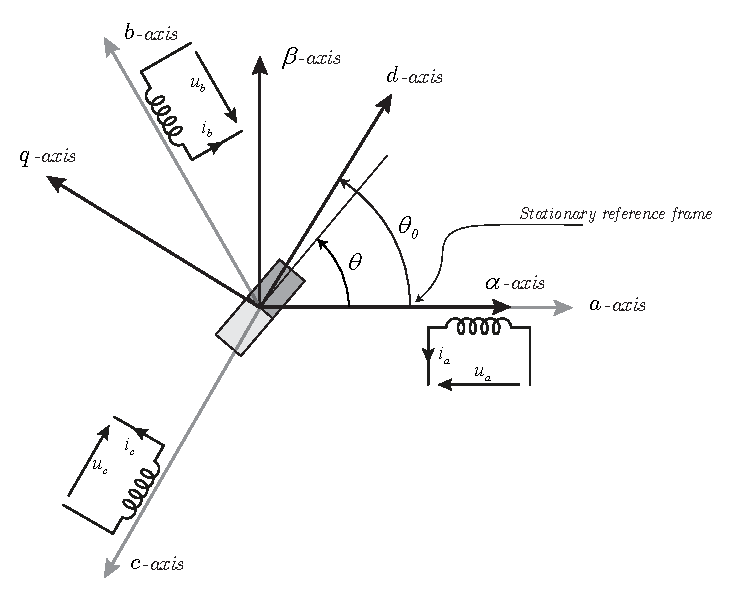
\includegraphics[width = 260pt, keepaspectratio]{figures/pmsm/reference_frames_dq.eps}
	\captionsetup{width=0.5\textwidth, font=small} 
	\caption	{Rotating $dq$ reference frame}
	\label{dq_ref_frame}
\end{figure}
Hence applying the transformation ${\mathbf{T}}_2(\vartheta_0)$ to the system represented by Eq.~\eqref{twophase_eq1} results as follows
\begin{equation*}
	\begin{aligned}
		\mathbf{T}_2^{-1}\vec{u}_{dq}-\mathbf{R}^{\alpha\beta}\ \mathbf{T}_2^{-1}\vec{i}_{dq}\ -\omega\frac{d\mathbf{L}_s^{\alpha\beta}}{d\theta}\mathbf{T}_2^{-1}\vec{i}_{dq}\ -\mathbf{L}^{\alpha\beta}\ \frac{d\left( \mathbf{T}_2^{-1}\vec{i}_{dq}\right) }{dt}-\frac{d\left( \mathbf{T}_2^{-1}\vec{\psi}_{dq}^{\,r}\right) }{dt} = 0
	\end{aligned} 
\end{equation*}
where
\begin{equation}
	\frac{d\mathbf{T}_2^{-1}(\vartheta_0)}{dt}= -\omega_0\begin{pmatrix} 0 & 1\\ -1 & 0 \end{pmatrix}\mathbf{T}_2^{-1}(\vartheta_0)
\end{equation}
left multiplying by $\mathbf{T}_2$ we obtain the following terms
\begin{equation}
	\begin{aligned}
		&-\mathbf{T}_2\mathbf{L}^{\alpha\beta}\ \frac{d\left( \mathbf{T}_2^{-1}\vec{i}_{dq}\right) }{dt} = \\[6pt]
		&=\omega_0\ \mathbf{T}_2\mathbf{L}^{\alpha\beta}\begin{pmatrix} 0 & 1\\ -1 & 0 \end{pmatrix}\mathbf{T}_2^{-1}\vec{i}_{dq}\ + \mathbf{T}_2\mathbf{L}^{\alpha\beta}\mathbf{T}_2^{-1}\frac{d\vec{i}_{dq}}{dt}  \\[6pt]
		&\xrightarrow{\theta_0\rightarrow\theta} \omega_0\begin{pmatrix} 0 & L_d\\ -L_q & 0 \end{pmatrix}\vec{i}_{dq}\ + \mathbf{L}^{dq}\frac{d\vec{i}_{dq}}{dt}
	\end{aligned}
\end{equation}
where 
\begin{equation}
	\begin{aligned}
		&\mathbf{L}^{dq} \xrightarrow{\theta_0\rightarrow\theta} \begin{pmatrix} L_d & 0\\ 0 & L_q \end{pmatrix} = \begin{pmatrix} L_{\mu}+\frac{3}{2}(L_a-L_b) & 0\\ 0 & L_{\mu}+\frac{3}{2}(L_a+L_b) \end{pmatrix}
	\end{aligned}
\end{equation}
and
\begin{equation}
	\begin{aligned}
		&-\omega\mathbf{T}_2\frac{d\mathbf{L}_s^{\alpha\beta}}{d\theta}\mathbf{T}_2^{-1}\vec{i}_{dq} = -\omega\mathbf{L}_m^{dq}\vec{i}_{dq}
		\xrightarrow{\theta_0\rightarrow\theta} \omega\begin{pmatrix} 0 & 3L_b\\ 3L_b & 0 \end{pmatrix}\vec{i}_{dq}\		
	\end{aligned}
\end{equation}
%and
%\begin{equation}
%	\begin{aligned}
%	&\mathbf{L}_m^{dq} \xrightarrow{\theta_0\rightarrow\theta} \begin{pmatrix} 0 & L_m^d\\ L_m^q & 0 \end{pmatrix} = \begin{pmatrix} 0 & -L_b\\ -L_b & 0 \end{pmatrix}
%\end{aligned}
%\end{equation}
Which results in the following set of equations
\begin{equation*}
	\left\lbrace \begin{aligned}
		& \vec{u}_{dq}-\mathbf{R}^{dq}\ \vec{i}_{dq} -\omega\mathbf{L}_m^{dq}\vec{i}_{dq} + \omega_0\begin{pmatrix} 0 & L_d\\ -L_q & 0 \end{pmatrix}\vec{i}_{dq} + \\[6pt] &\qquad\qquad-\mathbf{L}^{dq}\ \frac{d\vec{i}_{dq}}{dt} + \omega_0\,\begin{pmatrix} 0 & 1\\ -1 & 0 \end{pmatrix}\vec{\psi}_{dq}^{\,r} + (\omega - \omega_0)\begin{pmatrix} 0 & 1\\ -1 & 0 \end{pmatrix}\vec{\psi}_{dq}^{\,r} = 0\\[6pt]
		& \dot{\psi}_d^r = -\left( \omega-\omega_0\right)\psi_q^r \\[6pt]
		&\dot{\psi}_q^r = \left( \omega-\omega_0\right)\psi_d^r
	\end{aligned} \right. 
\end{equation*}
rearranging and approximating the term $\omega\mathbf{L}_m^{dq}\vec{i}_{dq}$ to 
$$-\omega\mathbf{L}_m^{dq}\vec{i}_{dq}
\xrightarrow{\theta_0\rightarrow\theta} \omega_0\begin{pmatrix} 0 & 3L_b\\ 3L_b & 0 \end{pmatrix}\vec{i}_{dq} = \omega\begin{pmatrix} 0 & L_q-L_d\\ L_q-L_d & 0 \end{pmatrix}\vec{i}_{dq}$$
we obtain the following set of equations  
\begin{equation}\label{eqdq}
	\left\lbrace \begin{aligned}
		& \vec{u}_{dq}-\mathbf{R}^{dq}\ \vec{i}_{dq} + \omega_0 \begin{pmatrix} 0 & L_q-L_d\\ L_q-L_d & 0 \end{pmatrix}\vec{i}_{dq} + \omega_0\begin{pmatrix} 0 & L_d\\ -L_q & 0 \end{pmatrix}\vec{i}_{dq} + \\[6pt]
		&\qquad\qquad-\mathbf{L}^{dq}\ \frac{d\vec{i}_{dq}}{dt} + \omega\begin{pmatrix} 0 & 1\\-1 & 0 \end{pmatrix}\vec{\psi}_{dq}^{\,r} = 0\\[6pt]
		& \dot{\psi}_d^r = -\left( \omega-\omega_0\right)\psi_q^r \\[6pt]
		&\dot{\psi}_q^r = \left( \omega-\omega_0\right)\psi_d^r 
	\end{aligned} \right. 
\end{equation}
recall that $3L_b=(L_q-L_d)$.

The flux equations in Eq.~\eqref{eqdq} are derived as follows
\begin{equation}
	\begin{aligned}
		& \frac{d\vec{\psi}^{\,r}_{\alpha\beta}(t)}{dt} = \omega(t) \begin{bmatrix} 0 & -1 \\ 1 & 0\end{bmatrix} \vec{\psi}^{\,r}_{\alpha\beta}(t) \Rightarrow \\[6pt]
		& \frac{d\mathbf{T}_2^{-1}\vec{\psi}^{\,r}_{dq}(t)}{dt} = \omega(t) \begin{bmatrix} 0 & -1 \\ 1 & 0\end{bmatrix} \mathbf{T}_2^{-1}\vec{\psi}^{\,r}_{dq}(t) \Rightarrow \\[6pt]
		&- \omega_0\begin{bmatrix} 0 & 1\\-1 & 0 \end{bmatrix}\mathbf{T}_2^{-1}\vec{\psi}_{dq} + \mathbf{T}_2^{-1}\frac{d\vec{\psi}^{\,r}_{dq}(t)}{dt} = \omega(t) \begin{bmatrix} 0 & -1 \\ 1 & 0\end{bmatrix} \mathbf{T}_2^{-1}\vec{\psi}^{\,r}_{dq}(t)
	\end{aligned}
\end{equation}
Multiplying both terms per $\mathbf{T}_2$ we obtain
\begin{equation}
	\begin{aligned}
		\frac{d\vec{\psi}^{\,r}_{dq}(t)}{dt} = \big(\omega-\omega_0\big)\begin{bmatrix} 0 & -1 \\ 1 & 0\end{bmatrix} \vec{\psi}^{\,r}_{dq}(t)
	\end{aligned}
\end{equation}
where $\vec{\psi}^{\,r}_{dq}(t)$ is given as follows
\begin{equation}
	\begin{aligned}
		\vec{\psi}^{\,r}_{dq}(t) = \mathbf{T}_2\vec{\psi}^{\,r}_{\alpha\beta} &= \begin{bmatrix} \cos(\theta_0) & \sin(\theta_0) \\[6pt] -\sin(\theta_0) & \cos(\theta_0) \end{bmatrix} \begin{bmatrix} \psi^m\cos(\theta_0) \\[6pt] \psi^m\sin(\theta_0) \end{bmatrix} = \\[6pt]
		&=\psi^m \begin{bmatrix} \cos\theta_0\cos\theta + \sin\theta_0\sin\theta \\[6pt] -\sin\theta_0\cos\theta+\cos\theta_0\sin\theta\end{bmatrix} =  \psi^m\begin{bmatrix} \cos\big(\theta -\theta_0\big) \\[6pt] \sin\big(\theta -\theta_0\big)\end{bmatrix}
	\end{aligned}
\end{equation}

Considering the $DQ$-classical control, we can observe that, when the rotating reference frame (which is the frame where the controller is implemented) and the rotor reference frame are aligned ($\theta_0 \rightarrow \theta$ and $\omega_0 \rightarrow \omega$), all the inductance matrices become time-invariant and the flux components become $\psi_{q} \rightarrow 0$, $\psi_{d} \rightarrow \psi^m$. 


\begin{mybox}
	\textbf{The DQ-PMSM model for a generic rotating reference frame is here reported}
	\begin{equation}\label{twophase_eq1bis}
		\left\lbrace \begin{aligned}
			& \vec{u}_{dq}-\mathbf{R}^{dq}\ \vec{i}_{dq} + \omega_0\begin{pmatrix} 0 & L_q\\ -L_d & 0 \end{pmatrix}\vec{i}_{dq} - \mathbf{L}^{dq}\ \frac{d\vec{i}_{dq}}{dt} + \omega\begin{pmatrix} 0 & 1\\-1 & 0 \end{pmatrix}\vec{\psi}_{dq}^{\,r} = 0\\[6pt]
			&\dot{\psi}_d^r = -\left( \omega-\omega_0\right)\psi_q^r \\[6pt]
			&\dot{\psi}_q^r = \left( \omega-\omega_0\right)\psi_d^r \\[6pt]
			& \vec{\psi}^{\,r}_{dq}(0) = \begin{bmatrix} \psi^m &  0 \end{bmatrix}^T \\[6pt]
			& J\dot{\omega}_m(t) = \tau_m(t)-b{\omega}_m-\tau_l(t) \\[6pt]
			& \dot{\vartheta}(t) = \omega(t) = p\omega_m(t)
		\end{aligned} \right. 
	\end{equation}
	where $\vec{\psi}^{\,r}_{dq} = \begin{bmatrix} \psi^m\cos(\theta-\theta_0) &  \psi^m\sin(\theta-\theta_0)\end{bmatrix}^T$ and
	\begin{equation*}
		\begin{aligned}
			& \mathbf{R}^{dq} = 
			\begin{bmatrix} R &  0 \\
				0 & R
			\end{bmatrix} \\[6pt]
			& \mathbf{L}^{dq} = 
			\begin{bmatrix} L_d &  0 \\
				0 & L_q
			\end{bmatrix} =
			\begin{bmatrix} L_\mu+\frac{3}{2}(L_a-L_b) &  0 \\
				0 & L_\mu+\frac{3}{2}(L_a+L_b)
			\end{bmatrix}
		\end{aligned} 
	\end{equation*}
	$\psi^m$ is the amplitude of the permanent magnet flux as viewed from the stator phase winding and we assume constant.
\end{mybox}

\begin{mybox}
	\textbf{The DQ-PMSM model, when rotating reference frame coincides with the rotor reference frame $\omega_0 \rightarrow \omega$, can be written as follows}
	\begin{equation}\label{twophase_eq2}
		\left\lbrace \begin{aligned}
			& \vec{u}_{dq}-\mathbf{R}^{dq}\ \vec{i}_{dq} - \mathbf{L}^{dq}\ \frac{d\vec{i}_{dq}}{dt} + \omega\begin{pmatrix} 0 & 1\\-1 & 0 \end{pmatrix}\vec{\psi}_{dq}^{\,s} = 0\\[6pt]
			&\dot{\psi}_d^s = -R_d i_d + \omega  \psi_q^s + u_d \\[6pt]
			&\dot{\psi}_q^s = -R_q i_q - \omega\psi_d^s + u_q \\[6pt]
			& \vec{\psi}^{\,r}_{dq}(0) = \begin{bmatrix} \psi^m &  0 \end{bmatrix}^T \\[6pt]
			& J\dot{\omega}_m(t) = \tau_m(t)-b{\omega}_m-\tau_l(t) \\[6pt]
			& \dot{\theta}(t) = \omega(t) = p\omega_m(t) 
		\end{aligned} \right. 
	\end{equation}
	where
	\begin{equation*}
		\begin{aligned}
			& \mathbf{R}^{dq} = 
			\begin{bmatrix} R &  0 \\
				0 & R
			\end{bmatrix} \\[6pt]
			& \mathbf{L}^{dq} = 
			\begin{bmatrix} L_d &  0 \\
				0 & L_q
			\end{bmatrix} =
			\begin{bmatrix} L_\mu+\frac{3}{2}(L_a-L_b) &  0 \\
				0 & L_\mu+\frac{3}{2}(L_a+L_b)
			\end{bmatrix}
		\end{aligned} 
	\end{equation*}
	$\psi^m$ is the amplitude of the permanent magnet flux as viewed from the stator phase winding and we assume constant.
\end{mybox}

\subsection{PMSM torque derivation}
\textbf{Torque equation of the isotropic PMSM - stationary reference frame}\\
Let $E$ be the stored energy inside of the PMSM, it can be described as follows
\begin{equation*}
	\begin{aligned}
		E = \frac{3}{2} \left(\frac{1}{2}\ \vec{i}_{\alpha\beta}^{\ T}\ \mathbf{L}^{\alpha\beta}\ \vec{i}_{\alpha\beta}\right) +\frac{1}{2}J\omega_m^2
	\end{aligned} 
\end{equation*}
Applying the principle of energy conservation we can write
\begin{equation*}
	\frac{dE}{dt} = 0
\end{equation*}
\begin{equation*}
	\frac{dE}{dt} = \frac{3}{2} \left( \vec{i}_{\alpha\beta}^{\ T}\ \mathbf{L}^{\alpha\beta}\ \frac{d\vec{i}_{\alpha\beta}}{dt}\right) + J\omega_m\dot{\omega}_m= P_{in}-P_{out}-P_{loss} = 0
\end{equation*}
We can write
\begin{equation*}
	\frac{3}{2} \left( \vec{i}_{\alpha\beta}^{\ T}\ \mathbf{L}^{\alpha\beta}\ \frac{d\vec{i}_{\alpha\beta}}{dt}\right) + J\omega_m\dot{\omega}_m =
\end{equation*}
\begin{equation*}
	=\frac{3}{2}\left( \underbrace{u_\alpha i_\alpha+u_\beta i_\beta}_{=\,P_{in}}-\underbrace{Ri_\alpha^2-Ri_\beta^2}_{=\,P_{loss}}-\underbrace{\omega 
		\begin{bmatrix} i_\alpha & i_\beta \end{bmatrix}
		\begin{bmatrix} 0 & -1 \\ 1 & 0\end{bmatrix}
		\begin{bmatrix} \psi^r_\alpha & \psi^r_\beta \end{bmatrix}^T
	}_{=\,\omega_m\tau_m}\right)  +\omega_m\tau_m-\omega_m\tau_l
\end{equation*}
But 
\begin{equation*}
	\frac{3}{2} \left( \vec{i}_{\alpha\beta}^{\ T}\ \mathbf{L}^{\alpha\beta}\ \frac{d\vec{i}_{\alpha\beta}}{dt}\right) + J\omega_m\dot{\omega}_m= P_{in}-P_{out}-P_{loss}
\end{equation*}
Hence
\begin{equation*}
	\begin{aligned}
		P_{in} &= \frac{3}{2}\left( u_\alpha i_\alpha+u_\beta i_\beta\right)  \\[6pt]
		P_{out} &= \omega_m\,\tau_l \\[6pt]
		P_{loss} &= \frac{3}{2}\left( Ri_\alpha^2+Ri_\beta^2\right) 
	\end{aligned} 
\end{equation*}
The expression of the torque $\tau_m$ becomes as follows
\begin{equation}
	\begin{aligned}
		\tau_m = \frac{3}{2}p\left( \psi^r_{\alpha}i_{\beta}-\psi^r_{\beta}i_{\alpha}\right) 
	\end{aligned} 
\end{equation}

\begin{mybox}
	\textbf{The full PMSM model respect to the stationary reference frame is as follows}
	\begin{equation}\label{twophase_model_ref}
		\left\lbrace \begin{aligned}
			& \vec{u}_{\alpha\beta}(t)-\mathbf{R}^{\alpha\beta}\ \vec{i}_{\alpha\beta}(t)-\mathbf{L}^{\alpha\beta}\ \frac{d\vec{i}_{\alpha\beta}(t)}{dt}-\omega(t) \begin{bmatrix} 0 & -1 \\ 1 & 0\end{bmatrix} \vec{\psi}^{\,r}_{\alpha\beta} = 0 \\[6pt]
			& \frac{d\vec{\psi}^{\,r}_{\alpha\beta}(t)}{dt} = \omega(t) \begin{bmatrix} 0 & -1 \\ 1 & 0\end{bmatrix} \vec{\psi}^{\,r}_{\alpha\beta}(t) \qquad \vec{\psi}^{\,r}_{\alpha\beta}(0) = \begin{bmatrix} \psi^m &  0 \end{bmatrix}^T \\[6pt]
			& J\dot{\omega}_m(t) = \frac{3}{2}p\Big[\psi^r_{\alpha}(t)i_{\beta}(t)-\psi^r_{\beta}(t)i_{\alpha}(t)\Big]-b\omega_m(t) -\tau_l(t) \\[6pt]
			& \dot{\theta}(t) = \omega(t) = p\omega_m(t)
		\end{aligned} \right. 
	\end{equation}
\end{mybox}

\textbf{Torque equation of the anisotropic PMSM - rotor reference frame}\\
Let $E$ be the stored energy inside of the PMSM, it can be described as follows
\begin{equation*}
	\begin{aligned}
		E = \frac{3}{2} \left(\frac{1}{2}\ \vec{i}_{dq}^{\ T}\ \mathbf{L}^{dq}\ \vec{i}_{dq}\right) +\frac{1}{2}J\omega_m^2
	\end{aligned} 
\end{equation*}
Applying the principle of energy conservation we can write
\begin{equation*}
	\frac{dE}{dt} = 0
\end{equation*}
\begin{equation*}
	\frac{dE}{dt} = \frac{3}{2} \left( \vec{i}_{dq}^{\ T}\ \mathbf{L}^{dq}\ \frac{d\vec{i}_{dq}}{dt}\right) + J\omega_m\dot{\omega}_m= P_{in}-P_{out}-P_{loss} = 0
\end{equation*}
We can write as follows
\begin{equation*}
	\frac{3}{2} \left( \vec{i}_{dq}^{\ T}\ \mathbf{L}^{dq}\ \frac{d\vec{i}_{dq}}{dt}\right) + J\omega_m\dot{\omega}_m =
\end{equation*}
\begin{equation*}
	\begin{aligned}
		&\underbrace{\frac{3}{2}\Big(u_d i_d+u_q i_q\Big)}_{=\,P_{in}}-\underbrace{\frac{3}{2}\Big(Ri_d^2-Ri_q^2\Big)}_{=\,P_{loss}} + \\[6pt]
		&-\underbrace{\frac{3}{2}\Big(\omega 
			\begin{bmatrix} i_d & i_q \end{bmatrix}
			\begin{bmatrix} 0 & -1 \\ 1 & 0\end{bmatrix}
			\begin{bmatrix} \psi^r_d & \psi^r_q \end{bmatrix}^T
			+\omega 
			\begin{bmatrix} i_d & i_q \end{bmatrix}
			\begin{bmatrix} 0 & -L_q \\ L_d & 0\end{bmatrix}
			\begin{bmatrix} i_d & i_q \end{bmatrix}^T\Big)
		}_{=\,\omega_m\tau_m} + \\[6pt]
		& +\omega_m\tau_m-\omega_m\tau_l
	\end{aligned}
\end{equation*}
But 
\begin{equation*}
	\frac{3}{2} \left( \vec{i}_{dq}^{\ T}\ \mathbf{L}^{dq}\ \frac{d\vec{i}_{dq}}{dt}\right) + J\omega\dot{\omega}= P_{in}-P_{out}-P_{loss}
\end{equation*}
Hence
\begin{equation*}
	\begin{aligned}
		P_{in} &= \frac{3}{2}\left( u_d i_d+u_q i_q\right)  \\[6pt]
		P_{out} &= \omega_m\,\tau_l \\[6pt]
		P_{loss} &= \frac{3}{2}\left( Ri_d^2+Ri_q^2\right) 
	\end{aligned} 
\end{equation*}
The expression of the torque $\tau_m$ becomes as follows
\begin{equation}
	\begin{aligned}
		\tau_m = \frac{3}{2}\,p\,\Big[\psi^r_{d}i_{q}-\psi^r_{q}i_{d} + \big(L_d-L_q\big)i_di_q\Big] \xrightarrow{\theta_0\rightarrow\theta} \frac{3}{2}\,p\,\Big[\psi^mi_{q} + \big(L_d-L_q\big)i_di_q\Big]
	\end{aligned} 
\end{equation}

\begin{mybox}
	\textbf{The full PMSM model respect to the rotor reference frame is as follows}
	\begin{equation}\label{twophase_model_ref_2}
		\left\lbrace \begin{aligned}
			& \vec{u}_{dq}(t)-\mathbf{R}^{dq}\ \vec{i}_{dq}(t)+ \omega\begin{bmatrix} 0 & L_q\\ -L_d & 0 \end{bmatrix}\vec{i}_{dq} -\mathbf{L}^{dq}\ \frac{d\vec{i}_{dq}(t)}{dt}-\omega(t) \begin{bmatrix} 0 & -1 \\ 1 & 0\end{bmatrix} \vec{\psi}^{\,r}_{dq} = 0 \\[6pt]
			& \frac{d\vec{\psi}^{\,r}_{dq}(t)}{dt} = 0 \qquad \vec{\psi}^{\,r}_{dq}(0) = \begin{bmatrix} \psi^m &  0 \end{bmatrix}^T \\[6pt]
			& J\dot{\omega}_m(t) = \frac{3}{2}\,p\,\Big[\psi^mi_{q} + \big(L_d-L_q\big)i_di_q\Big] -b\omega_m(t)-\tau_l(t) \\[6pt]
			& \dot{\theta}(t) = \omega(t) = p\omega_m(t)
		\end{aligned} \right. 
	\end{equation}
\end{mybox}
\subsection{Equivalent circuit of a PMSM}
The DQ equivalent circuits of the PMSM is shown for both transient and steady state conditions.
\begin{figure}[H]
	\centering
	\begin{subfigure}{.5\textwidth}
		\centering
		\includegraphics[width = 200pt, keepaspectratio]{figures/pmsm/pmsm_electrical_equivalent_1.eps}
		\captionsetup{width=0.5\textwidth, font=small}		
		\caption{PMSM equivalent circuit for the generic rotating reference frame case.}
		\label{}
	\end{subfigure}%
	\begin{subfigure}{.5\textwidth}
		\centering
		\includegraphics[width = 200pt, keepaspectratio]{figures/pmsm/pmsm_electrical_equivalent_2.eps}
		\captionsetup{width=0.5\textwidth, font=small}		
		\caption{PMSM equivalent circuit for the rotor reference frame case.}
		\label{}
	\end{subfigure}
	\captionsetup{width=0.5\textwidth, font=small}		
	\caption{Rotating and rotor reference frame representation of the pmsm equivalent circuit.}
	\label{pmsm_equivalent_circuit}
\end{figure}

\section{Control of a PMSM}
The structure of the PMSM control is based on the following parts:
\begin{itemize}
	\item Speed control.
	\item Torque control based on current vector control in DQ reference frame.
	\item MTPA
	\item Field weakening
\end{itemize}

\subsection{Classical Field Oriented Control of a PMSM}
The classical field oriented control (FOC) DQ-control of PMSMs in Figure~\ref{pmsm_class_ctrl_1} is depicted.
\begin{figure}[H]
	\centering
	\includegraphics[width = 400pt, keepaspectratio]{figures/pmsm/pmsm_foc_ctrl_scheme_1.eps}
	\captionsetup{width=0.5\textwidth, font=small}
	\caption{Global vector control of the classical of a PMSM.}
	\label{pmsm_foc_ctrl_scheme_1}
\end{figure}
\begin{figure}[H]
	\centering
	\includegraphics[width = 500pt, keepaspectratio]{figures/pmsm/pmsm_classical_ctrl_2.eps}
	\captionsetup{width=0.5\textwidth, font=small}
	\caption{Internal current control of the classical FOC of a PMSM.}
	\label{pmsm_class_ctrl_1}
\end{figure}


The \textbf{FOC} control strategy is based on the control of two current components. The two current components ($i_d,\,i_q$) are derived by a proper transformation of the PMSM three phase current system into the $dq$ reference frame. The knowledge of the rotor phase $\theta$ plays a fundamental role in the performance of the control system. A perfect knowledge of the rotor position $\theta$ permits to decouple the control system into two current component where the $Q$ axis concerns the generation of the torque and the $D$ axis affect the value of the terminal voltage and can be properly set in order to extend the working operative are of the PMSMs as shown in Figure~\ref{vector_plane_1}.
\begin{figure}[H]
	\centering
	\includegraphics[width = 400pt, keepaspectratio]{figures/pmsm/pmsm_vector_graph_1.eps}
	\captionsetup{width=0.5\textwidth, font=small}
	\caption{Vector diagram of the PMSM and effect of the $i_d$ current component on the terminal voltage $\vec{v}_g$.}
	\label{vector_plane_1}
\end{figure}
\subsection{Normalization and control implementation.}
Concerning the model representation and the control implementation we in front of two completely different approach. A model implementation is, in general, represented in SI unit and often in continuous time domain. On the other hand a control system as well as the state space representation of the dynamical system of the plant is, often, represented in per unit and in discrete time domain. The representation in per unit given many advantages in term of usability and \textit{control gain} stability among different plants implementations.

The per unit representation of the model pass through the \textit{normalization}, as follows
\begin{itemize}
	\item[--] Reference quantities
	\begin{itemize}
		\item[--] $u_{bez} = $ is the peak phase voltage of the no-load voltage at nominal rotor speed $\omega_m^{nom}$ of the motor in $\SI{}{\volt}$ and can be derived from parameter $K_e$ (Voltage Constant) as well as from parameter $K_t$ (Torque Constant) as follows
		\begin{equation}
			u_{bez} = \psi^m\omega_{bez} 
		\end{equation}
	where
		\begin{equation}
			\begin{aligned}
			& \psi^m = K_e\quad \text{or} \\[6pt]
			& \psi^m = K_t\frac{\sqrt{2}}{3p} \qquad\text{we consider $i_d=0$ control}
			\end{aligned}
		\end{equation}
		\item[--] $i_{bez} = $ is the peak phase nominal current of the motor in $\SI{}{\ampere}$ and can be derived from parameter $\tau_m^{nom}$ (Nominal Torque) as follows
		\begin{equation}
			i_{bez} = \frac{\tau_m^{nom}}{K_t}\sqrt{2} \qquad\text{we consider $i_d=0$ control}
		\end{equation}
		\item[--] $\omega_m^{nom} = $ is the nominal mechanical rotor speed of the motor in $\SI{}{\radian\per\second}$
		\item[--] $\omega_{bez} = p \omega_m^{nom}$ is the nominal electrical speed of the motor in $\SI{}{\radian\per\second}$
		\item[--] $X_{bez} = u_{bez}/i_{bez} = $ is the reference electrical impedance of the motor in $\SI{}{\ohm}$
		\item[--] $L_{bez} = X_{bez}/\omega_{bez} = $ is the reference inductance of the motor in $\SI{}{\henry}$	
		\item[--] $\psi_{bez} = u_{bez}/\omega_{bez} = $ is the reference flux of the motor in $\SI{}{\weber}$
	\end{itemize}
	\item[--] Per unit quantities
		\begin{itemize}
		\item[--] $R^{norm} = R/X_{bez}$ is the per unit phase resistance.
		\item[--] $L_d^{norm} = L_d/L_{bez}$ is the per unit phase $L_d$ inductance.
		\item[--] $L_q^{norm} = L_q/L_{bez}$ is the per unit phase $L_q$ inductance.
		\item[--] $\omega^{norm} = p\omega_m/\omega_{bez}$ is the per unit electrical speed.		
		\item[--] $i_d^{norm} = i_d/i_{bez}$ is the per unit $i_d$ current.
		\item[--] $i_q^{norm} = i_q/i_{bez}$ is the per unit $i_q$ current.
		\item[--] $u_d^{norm} = u_d/u_{bez}$ is the per unit $u_d$ voltage.
		\item[--] $u_q^{norm} = u_q/u_{bez}$ is the per unit $u_q$ voltage.		
		\item[--] $\psi_d^{norm} = \psi_d/\psi_{bez}$ is the per unit D-flux.
		\item[--] $\psi_q^{norm} = \psi_q/\psi_{bez}$ is the per unit Q-flux.
		\item[--] $\psi_m^{norm} = \psi^m/\psi_{bez}$ is the per unit M-flux.
		\end{itemize}	 
\end{itemize}
and the FOC control implementation become (in continuous time domain) - in the following we omit the term $\Big(^{norm}\Big)$ and we consider all as per unit quantities
\begin{mybox}
\begin{equation}
	\left\lbrace \begin{aligned}
		&i_q^{ref} = k_p^w\Big(\omega^{ref} - \omega\Big) + i_{q}^{i} \\[6pt]
		&\frac{d}{dt} i_{q}^{i}= k_i^w\Big(\omega^{ref} - \omega\Big) \\[6pt]
		&u_d =  k_p^i\Big(i_d^{ref} - i_d\Big) + u_d^i - \omega\hat{\psi}_q - \omega L_q i_q \\[6pt]
		&\frac{d}{dt} u_d^i= k_i^i\Big(i_d^{ref} - i_d\Big)\\[6pt]
		&u_q =  k_p^i\Big(i_q^{ref} - i_q\Big) + u_d^i + \omega\hat{\psi}_d - \omega L_d i_d \\[6pt]
		&\frac{d}{dt} u_q^i= k_i^i\Big(i_q^{ref} - i_q\Big)
	\end{aligned}\right. 
\end{equation}
\end{mybox}

\subsection{PMSM current loci and over-speed management}
The control of a PMSM and in particular of an IPMSM where $L_d$ and $L_q$ are strongly different, has some degree of freedom concerning the set-point of the current $i_d$. As we will see, the current $i_d$ can be used to coercive the terminal voltage (flux weakening, FW) of PMSM (which is subjected to the inverter constraints) to a given value. Moreover the a proper set of $i_d$ current can be selected to optimize some properties of the PMSM like the maximum torque per ampere (MTPA) or the maximum torque per voltage (MTPV), or to minimize the copper power losses, or in flux weakening, etc.
\begin{figure}[H]
	\centering
	\includegraphics[width = 400pt, keepaspectratio]{figures/pmsm/pmsm_vector_graph_2.eps}
	\captionsetup{width=0.5\textwidth, font=small}
	\caption{Vector diagram of the PMSM and effect of the $i_d$ current component on the terminal voltage $\vec{v}_g$ - Field weakening case.}
	\label{vector_plane_2}
\end{figure}
In general an IPMSM is controlled by the MTPA and when it reach the maximum voltage (due to over-speed) the current loci $i_d-i_q$ can be kept along a maximum voltage curve until a maximum current (circle - $i_d-i_q$) is reached. When the current loci lays in a maximum current curve, the control can move along the limit curve until a different control strategy, like MTPV is adopted.
\begin{figure}[H]
	\centering
	\includegraphics[width = 360pt, keepaspectratio]{figures/deflux/deflux_bianchi_3b.eps}
	\captionsetup{width=0.5\textwidth, font=small}
	\caption{Current limit circle and voltage limit ellipses in $i_d-i_q$ plane.}
	\label{deflux_1}
\end{figure}
Another very common control strategy is the $i_d=0$ control, obviously this control is naturally the best choice for isotropic PMSM ($L_d=L_q$), even if is widely used in IPMSM. Using $i_d=0$ control in a IPMSM de-rate the effective efficiency of the system, requiring more current than what can be used in the case of a MTPA control.

Some current loci are shown in Figures~\ref{deflux_1} and~\ref{deflux_2}
\begin{figure}[H]
	\centering
	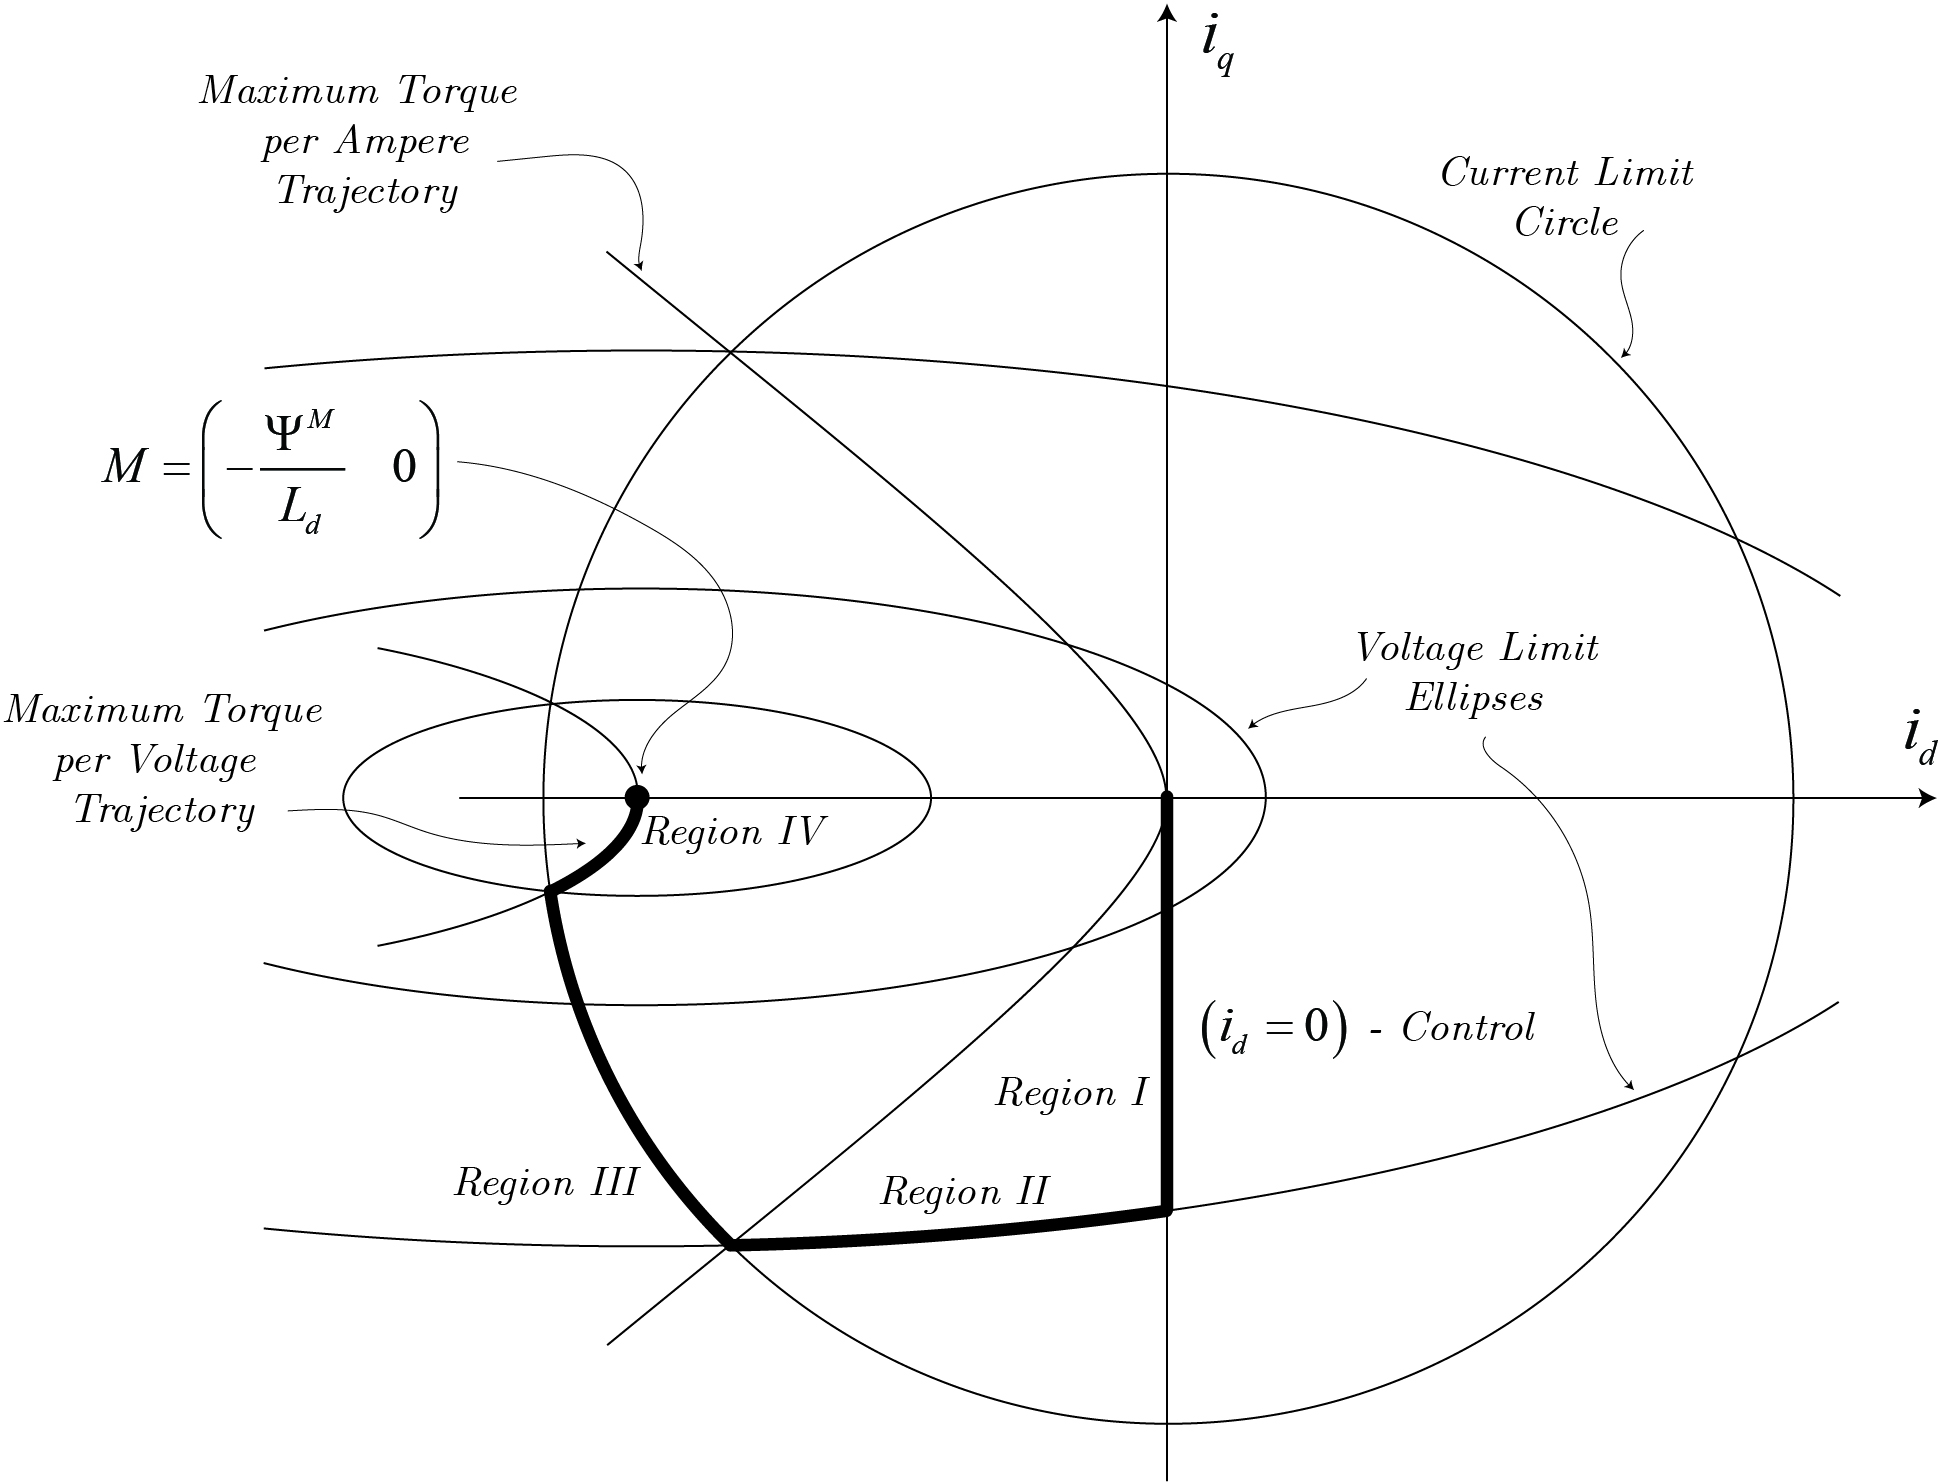
\includegraphics[width = 400pt, keepaspectratio]{figures/deflux/deflux_bianchi_9.jpg}
	\captionsetup{width=0.5\textwidth, font=small}
	\caption{Some possible current control strategies and their properties.}
	\label{deflux_2}
\end{figure}
The relation between $d$-axis and $q$-axis currents for the \textbf{maximum torque per ampere} (MTPA) condition is given as follows
\begin{equation}
	\left\lbrace \begin{aligned}
	&i_d^{ref} = \frac{\hat{\psi}^m(t)}{2\Big(L_q-L_d\Big)}-\sqrt{\frac{\Big(\hat{\psi}^m(t)\Big)^2}{4\Big(L_q-L_d\Big)^2}+i_q^2} \\[6pt]
	&i_q^{ref} = \quad\text{as per torque}
		\end{aligned}\right. 
\end{equation}
for PMSM with stable permanent magnet linkage flux, and to avoid additional dynamics from flux state observer, the following implementation can also be adopted:
\begin{equation}
	\left\lbrace \begin{aligned}
		&\hat{\psi}^m(t) \rightarrow \psi_m^{bez} \\[6pt]
		&i_d^{ref} = \frac{\psi_m^{bez}}{2\Big(L_q-L_d\Big)}-\sqrt{\frac{\Big(\psi_m^{bez}\Big)^2}{4\Big(L_q-L_d\Big)^2}+i_q^2} \\[6pt]
		&i_q^{ref} = \quad\text{as per torque}
	\end{aligned}\right. 
\end{equation}

The optimal current vector by which the torque per flux linkage $\psi_0 = \sqrt{\Big(\psi^m+L_di_d \Big) + \Big(L_qi_q\Big)^2}$ become maximal is given as follows
\begin{equation}\label{bianchi_1}
	\left\lbrace \begin{aligned}
		&i_d=-\frac{\psi^m+\Delta \psi_d^r}{L_d} \\[6pt]
		&i_q=\frac{1}{L_q}\sqrt{\Big(\psi_0 \Big)^2-\Big(\Delta\psi_d^r \Big)^2}
	\end{aligned}\right. 
\end{equation}
where 
\begin{equation}\label{bianchi_2}
	\begin{aligned}
		&\Delta \psi_d^r = \frac{-L_q\psi^m+\sqrt{\Big(L_q\psi^m\Big)^2+8\Big(L_q-L_d\Big)^2\psi_0^2}}{4\big(L_q-L_d\big)}
	\end{aligned}
\end{equation}
The vector control based on Eq.~\eqref{bianchi_1} and~\ref{bianchi_2} can be called \textit{the maximum torque per flux linkage (MTPF) control}. This condition is equal to maximizing the torque to the voltage $v_g$, where  $v_g$ is defined as follows 
\begin{equation}\label{bianchi_3}
	\begin{aligned}
		&v_g = \sqrt{\Big(\omega\psi^m + Ri_q + \omega L_d i_d\Big)^2 + \Big(Ri_d - \omega L_q i_q\Big)^2}
	\end{aligned}
\end{equation}
thus this vector control is named \textit{the maximum torque per voltage (MTPV) control}. 

One of the most interesting and important $i_d-i_q$ current loci is the \textit{constant voltage} locus, where in Figure~\ref{deflux_2} is described like a ellipses. This current loci is very important and widely used in \textbf{generator mode} where the speed motor is imposed by the external system. Along this region (\textit{region II}) the output voltage of the inverter (or of the terminals of the PMSM) is kept constant (in modulus) and the current vector is not more controlled but is free to rotate or move along this ellipses. This region is often used as \textbf{self field weakening control}, in fact, we can observe that in this condition the inverter is able to keep loaded the PMSM by automatically rotation of the motor current (the current is rotating out of control) in order to maintain the modulus of the terminal voltage constant and modifying the actual torque.

\subsection{Robust field weakening control architecture}
In this section a feedback (closed loop) field weakening control structure is proposed. 

\begin{figure}[H]
	\centering
	\includegraphics[width = 450pt, keepaspectratio]{figures/deflux/closed_loop_fw_1.eps}
	\captionsetup{width=0.5\textwidth, font=small}
	\caption{Robust flux weakening control architecture.}
	\label{}
\end{figure}

\section{Parameters identification}
PMSM parameters can be determined from datasheet and factory tests which in general are available from supplier. In order to characterize the motor the following data shall be collected:
\begin{itemize}
		\item[$-$] \textbf{Number of poles.}
		\item[$-$] \textbf{Nominal data.}
	\begin{itemize}
		\item[$-$] Nominal speed.
		\item[$-$] Nominal current.
		\item[$-$] Nominal voltage.
		\item[$-$] Nominal torque.
	\end{itemize}
	\item[$-$] \textbf{No-load voltage test.}
	\item[$-$] \textbf{Terminals short circuit test.}
	\item[$-$] \textbf{Measure of the stator phase resistance.}
\end{itemize}
In order to identify correctly the values of $L_d$ and $L_q$ which can affect considerably the performance of MTPA (for anisotropic permanent magnet motor as IPMSM) additional test can be carried out as in the next will be explained.

\subsection{No-load test}
The \textbf{no-load test} in one of the most important test in order to characterize the model of the PMSM. The no-load test consists to run the motor without any load at nominal speed. In this condition the load current is very low and completely negligible. In this condition the terminal phase voltages correspond to the back emf 
\begin{equation}
	\vec{E}=-\frac{d\psi^r(t)}{dt}=\begin{bmatrix} \omega\psi^m\sin(\vartheta) \\[6pt] \omega\psi^m\sin(\vartheta-2\pi/3) \\[6pt] \omega\psi^m\sin(\vartheta +2\pi/3)\end{bmatrix}
\end{equation}
That means by the no-load test permanent magnet flux linkage $\psi^m(t)$ can be determined. During the no-load test the voltage vector $\vec{E}$ is measured and the frequency $\omega$ is known.

\subsection{Terminals short circuit test}
From \textbf{terminals short circuit test} the value of $L_d$ can approximately determined. During these test the equivalent model of the PMSM can represented as shown in Figure~\ref{TerminalsShortCircuitTest} where the voltage drop across the phase resistance has been considered negligible.
\begin{figure}[H]
	\centering
	\includegraphics[width = 260pt, keepaspectratio]{figures/pmsm/TerminalsShortCircuitTest.eps}
	\captionsetup{width=0.5\textwidth, font=small}
	\caption{Terminals short circuit test from electrical point of view.}
	\label{TerminalsShortCircuitTest}
\end{figure}
Measuring the phase current $i_{ph}=i_d$ and knowing the back emf voltage from no-load test is it possible to determine the value of inductance $L_d = \frac{\psi^m}{i_d}$. 

\subsection{Load test}
Load test is one of the mandatory test which have to be performed. This test results in a very wide range of information results, from thermodynamic behavior to internal machine behavior. 

For MTPA the knowledge of both $L_d$ and $L_q$ must be known. The inductance value $L_q$ can be determined from the comparison of the terminal voltage at different loads. In this contest the load test (at different loads) can be used for this purpose.
\begin{figure}[H]
	\centering
	\includegraphics[width = 400pt, keepaspectratio]{figures/pmsm/load_test_Lq.eps}
	\captionsetup{width=0.5\textwidth, font=small}
	\caption{Load test and method to determine the $L_q$ inductance.}
	\label{load_test_Lq}
\end{figure}
From Figure~\ref{load_test_Lq} we can se that the terminal voltage DQ components $\vec{v}_{g}=\begin{bmatrix} v_d^g &  v_q^g \end{bmatrix}^T$ can be written as follows
\begin{equation}
	\left\lbrace \begin{aligned}
	&	v_d^g = \omega L_q i_q \\[6pt]
	&	v_q^g = \omega \psi^m
	\end{aligned}\right. 
\end{equation}
by the knowledge of the rotor position $\vartheta$ is it possible to measure the voltage components $\begin{bmatrix} v_d^g &  v_q^g \end{bmatrix}^T$ and hence the value of $L_q$ at different load conditions.

\section{Model parameters settings}

\begin{itemize}
	\item[$-$] Mode of operation
	\item[$-$] Motor parameters
	\item[$-$] Control parameters
\end{itemize} 

\textbf{Mode of operation} consists of the following parameters
\begin{itemize}
	\item[$-$] \textbf{Enable Speed Mode}
	\begin{itemize}
		\item[$-$] \textbf{Speed Mode}: Motor is controlled in speed mode. A speed set-point has to be set.
		\item[$-$] \textbf{Torque Mode}: Motor is controlled in torque mode. A torque set-point has to be. set.		
	\end{itemize}
	\item[$-$] \textbf{Enable Speed Mode}: if speed mode is enabled
		\begin{itemize}
			\item[$-$] \textbf{Torque limited from torque reference}: A maximum torque set-point has to be provide.
			\item[$-$] \textbf{Torque unlimited}: Motor behaves as an ideal speed source.
		\end{itemize}
\end{itemize}

\textbf{Motor parameters} consists of the following parameters
\begin{itemize}
	\item[--] \textbf{Number of motor pole pairs}: is the number of motor pole pairs.
	\item[--] \textbf{Maximum Speed} $\omega_m^{max}[\SI{}{\per\minute}]$: is the motor maximum speed (mechanical).	\item[--] \textbf{Nominal Speed} $\omega_m^{nom}[\SI{}{\per\minute}]$: is the motor nominal speed (mechanical).
	\item[--] \textbf{Nominal Torque} $\tau_m^{nom}[\SI{}{\newton\meter}]$: is the motor nominal torque.
	\item[--] \textbf{Phase Resistance} $R_{s}[\SI{}{\ohm}]$: is the nominal stator phase resistance.
	\item[--] \textbf{D-inductance} $L_{d}[\SI{}{\henry}]$: is the direct axis inductance.
	\item[--] \textbf{Q-inductance} $L_{q}[\SI{}{\henry}]$: is the quadrature axis inductance.
	\item[--] \textbf{Voltage Constant} $K_e[\SI{ }{\volt\second\per\radian}]$: Neutral-phase voltage peak per electrical pulsation.
	\item[--] \textbf{Torque Constant} $K_t[\SI{ }{\newton\meter\per\ampere_\text{rms}}]$: Torque per ampere rms.
	\item[--] \textbf{Rotor Inertia} $J_m[\SI{}{\kilo\gram\square\meter}]$: is the nominal rotor mechanical inertia.
	\item[--] \textbf{Rotor Friction} $b[\SI{}{\newton\meter\per{\radian\per\second}}]$: is the bearing viscosity.
\end{itemize}

\textbf{Motor parameters} consists of the following parameters
\begin{itemize}
	\item[$-$] \textbf{Proportional Speed Ctrl Gain} $k_p^\omega$
	\item[$-$] \textbf{Integral Speed Ctrl Gain} $k_i^\omega$
	\item[$-$] \textbf{Proportional Current Ctrl Gain} $k_p^i$
	\item[$-$] \textbf{Integral Current Ctrl Gain} $k_i^i$
	\item[$-$] \textbf{Proportional Field Weakening Ctrl Gain} $k_p^{fw}$
	\item[$-$] \textbf{Integral Field Weakening Ctrl Gain} $k_i^{fw}$
\end{itemize}

\section{Model output variables}
The output bus channel \textbf{PMSM data} includes the following data output
\begin{itemize}
	\item[$-$] $\omega_m$: mechanical speed $\Big[\SI{}{\per\minute}\Big]$.
	\item[$-$] $\tau_m$: electromagnetic torque $\Big[\SI{}{\newton\meter}\Big]$.
	\item[$-$] $i_g$: phase current in rms $\Big[\SI{}{\ampere_\text{rms}}\Big]$.	
	\item[$-$] $i_d$: direct current $\Big[\SI{}{\ampere}\Big]$.	
	\item[$-$] $i_q$: quadrature current $\Big[\SI{}{\ampere}\Big]$.
	\item[$-$] $\psi_d^s=\psi_d^r+i_dL_d$: direct flux $\Big[\SI{}{\weber}\Big]$.	
	\item[$-$] $\psi_q^s=\psi_q^r+i_qL_q$: quadrature flux $\Big[\SI{}{\weber}\Big]$.	
	\item[$-$] $e_d$: direct back EMF component $\Big[\SI{}{\volt}\Big]$.	
	\item[$-$] $e_q$: quadrature back EMF component $\Big[\SI{}{\volt}\Big]$.
	\item[$-$] $v_g$: phase to phase terminal voltage in rms $\Big[\SI{}{\volt_\text{rms}}\Big]$.		
	\item[$-$] $u_d$: direct terminal voltage component $\Big[\SI{}{\volt}\Big]$.	
	\item[$-$] $u_q$: quadrature terminal voltage component $\Big[\SI{}{\volt}\Big]$.
	\item[$-$] $P_{in}$: Active power at motor terminal $\Big[\SI{}{\kilo\watt}\Big]$.	
\end{itemize}

\begin{thebibliography}{99}

	\bibitem[\textbf{P. Krause, 2013}]{p4} P. Krause, O. Wasynczuk, S. Sudhoff, S. Pekarek - \textit{Analysis of Electric Machinery and Drive Systems}. Wiley 2013.
			
	\bibitem[\textbf{N. Bianchi, 2004}]{p10} N. Bianchi, T. Jahns - \textit{Design, analysis, and control of interior PM synchronous machines}. CLEUP 2004.
	
\end{thebibliography}
\end{onehalfspace}
\end{document} 